\documentclass[aspectratio=169,10pt]{beamer}

\usetheme{Madrid}
\usecolortheme{seahorse}

\usepackage[utf8]{inputenc}
\usepackage{amsmath}
\usepackage{amssymb}
\usepackage{amsfonts}
\usepackage{mathtools}
\usepackage{amsthm}
\usepackage{xcolor}
\usepackage{listings}
\usepackage{xkeyval}
\usepackage{tikz}
\usetikzlibrary{shapes,arrows,positioning}

\graphicspath{{figures/}}

\definecolor{codegreen}{rgb}{0,0.6,0}
\definecolor{codegray}{rgb}{0.5,0.5,0.5}
\definecolor{codepurple}{rgb}{0.58,0,0.82}
\definecolor{backcolour}{rgb}{0.95,0.95,0.92}

\lstdefinestyle{pythonstyle}{
    backgroundcolor=\color{backcolour},
    commentstyle=\color{codegreen}\itshape,
    keywordstyle=\color{codepurple}\bfseries,
    numberstyle=\tiny\color{codegray},
    stringstyle=\color{codepurple},
    basicstyle=\ttfamily\scriptsize,
    breakatwhitespace=false,
    breaklines=true,
    captionpos=b,
    keepspaces=true,
    numbers=left,
    numbersep=5pt,
    showspaces=false,
    showstringspaces=false,
    showtabs=false,
    tabsize=2,
    frame=single,
    rulecolor=\color{black}
}

\lstset{style=pythonstyle}

% Define remark environment for Beamer
\makeatletter
\newenvironment{remark}[1][]{\begin{block}{Remark \ifx\relax#1\relax\else~(#1)\fi}}{\end{block}}
\makeatother

\setbeamertemplate{footline}[frame number]
\setbeamertemplate{navigation symbols}{}

\title[Nonlinear Complementarity Problems]{Nonlinear Complementarity Problems}
\subtitle{Chapter 8e: Applications and Theory}
\author{Based on Pathak's \textit{Nonlinear Analysis and Fixed Point Theory}}
\date{\today}

\begin{document}

% ============================================================================
% TITLE SLIDE
% ============================================================================
\begin{frame}
\titlepage
\end{frame}

% ============================================================================
% OUTLINE
% ============================================================================
\begin{frame}[fragile]
\frametitle{Chapter Outline}

\begin{enumerate}
    \item \textbf{Introduction and Motivation}
    \begin{itemize}
        \item Historical development and applications
        \item Problem formulations
    \end{itemize}

    \item \textbf{Complementarity Problem Formulations}
    \begin{itemize}
        \item Explicit Complementarity Problem (E.C.P)
        \item Implicit Complementarity Problem (I.C.P)
        \item Simultaneous versions (S.E.C.P, S.I.C.P)
    \end{itemize}

    \item \textbf{Theoretical Framework}
    \begin{itemize}
        \item Cones and dual cones
        \item n-Lipschitz and n-strongly monotone mappings
    \end{itemize}

    \item \textbf{Main Existence and Uniqueness Results}
    \begin{itemize}
        \item Theorem 9.39 (Pathak et al.)
        \item Solution methods and convergence
    \end{itemize}

    \item \textbf{Applications and Examples}
    \begin{itemize}
        \item Optimization problems
        \item Engineering and economic applications
    \end{itemize}
\end{enumerate}

\end{frame}

% ============================================================================
% SECTION 1: INTRODUCTION
% ============================================================================
\section{Introduction and Motivation}

\begin{frame}
\frametitle{Historical Development of Complementarity Problems}

\begin{itemize}
    \item \textbf{Origins (1960s):} Complementarity problems emerged in the context of mathematical programming and optimization

    \item \textbf{Key Contributors:}
    \begin{itemize}
        \item Cottle, Lemke: Linear complementarity problems
        \item Karamardian: Nonlinear complementarity theory
        \item Pang, Ferris: Variational inequality connections
    \end{itemize}

    \item \textbf{Motivations:}
    \begin{itemize}
        \item Optimization with constraints
        \item Economic equilibrium problems
        \item Contact mechanics and engineering
        \item Structural analysis and elasticity
    \end{itemize}

    \item \textbf{Modern Applications:}
    \begin{itemize}
        \item Machine learning: Support vector machines
        \item Game theory: Nash equilibrium
        \item Variational inequalities
        \item Friction and contact problems in mechanics
    \end{itemize}
\end{itemize}

\end{frame}

\begin{frame}
\frametitle{Wide Range of Applications}

Complementarity problems have applications in:

\begin{columns}[T]
\column{0.5\textwidth}
\textbf{Optimization Theory}
\begin{itemize}
    \item Constrained optimization
    \item Convex analysis
    \item Nonconvex optimization
\end{itemize}

\textbf{Engineering}
\begin{itemize}
    \item Structural mechanics
    \item Elasticity theory
    \item Lubrication theory
\end{itemize}

\column{0.5\textwidth}
\textbf{Economics and Game Theory}
\begin{itemize}
    \item Economic equilibrium
    \item Game theory
    \item Market equilibrium
\end{itemize}

\textbf{Variational Problems}
\begin{itemize}
    \item Variational inequalities
    \item Differential equations
    \item Control theory
\end{itemize}
\end{columns}

\vspace{0.3cm}

\centering
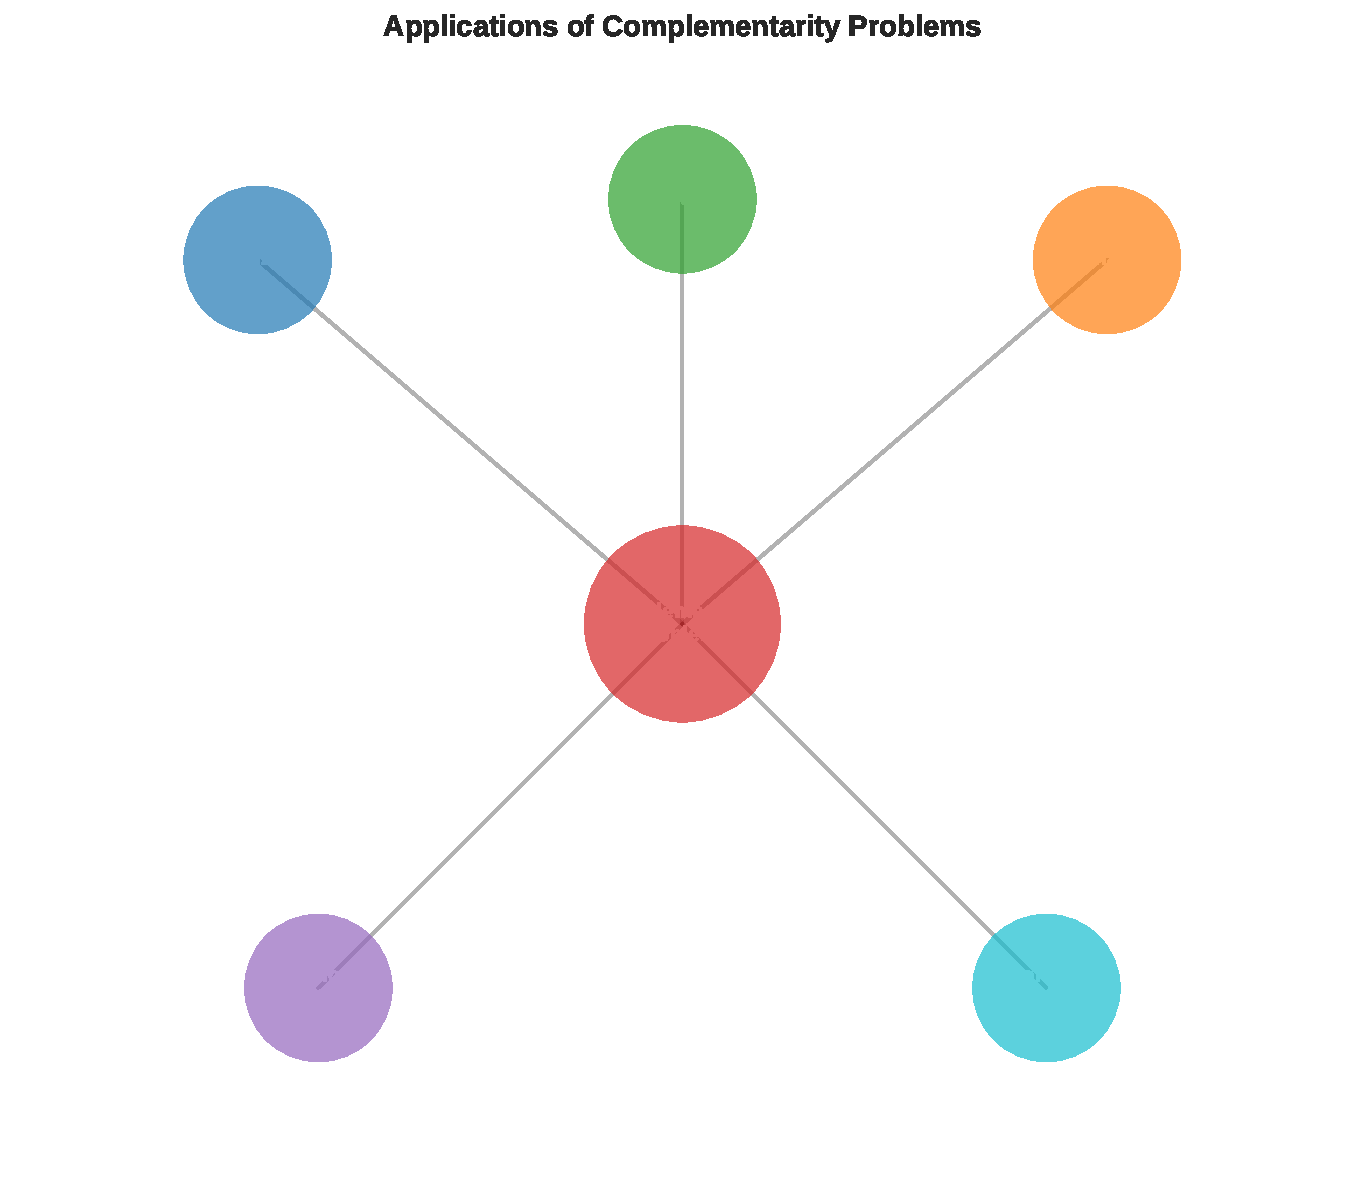
\includegraphics[width=0.8\textwidth]{06_applications.pdf}

\end{frame}

% ============================================================================
% SECTION 2: BASIC CONCEPTS
% ============================================================================
\section{Basic Concepts and Definitions}

\begin{frame}
\frametitle{Cones and Dual Cones}

\begin{definition}
Let $E$ be a locally convex space and $K \subseteq E$ a \textbf{closed convex cone}:
\begin{align*}
K^* = \{u \in E^* : \langle u, x \rangle \geq 0 \text{ for all } x \in E\}
\end{align*}
is called the \textbf{dual cone} or \textbf{polar cone} of $K$.
\end{definition}

\vspace{0.3cm}

\textbf{Key Properties:}
\begin{itemize}
    \item $K^*$ is always a closed convex cone
    \item If $K$ is a closed convex cone, then $(K^*)^* = K$
    \item For the positive orthant: $({\mathbb{R}}^n_+)^* = {\mathbb{R}}^n_+$
\end{itemize}

\vspace{0.3cm}

\centering
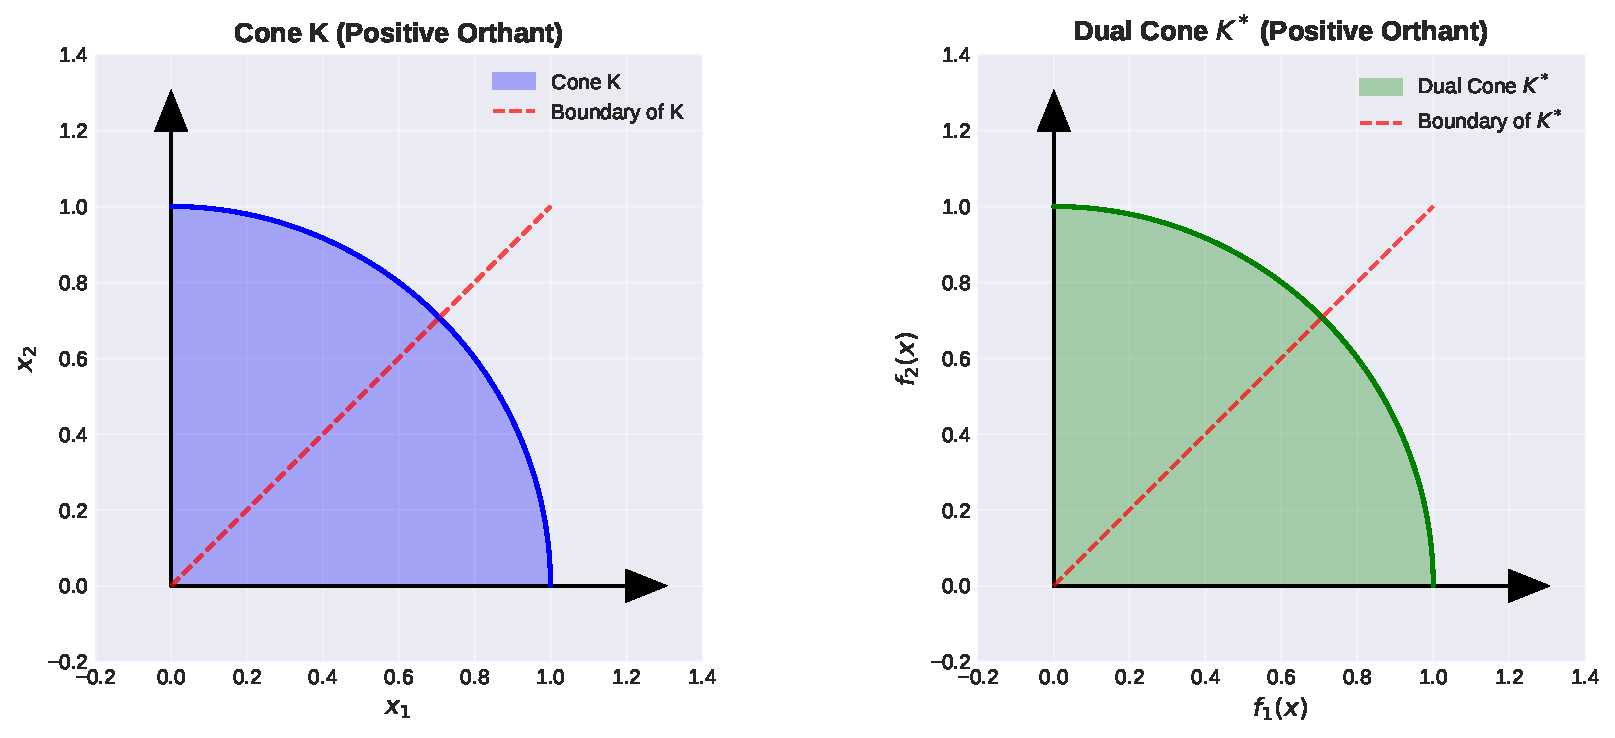
\includegraphics[width=0.9\textwidth]{01_cone_dual_cone.pdf}

\end{frame}

\begin{frame}
\frametitle{Complementarity Condition}

\begin{definition}
Let $K$ be a closed convex cone in a Hilbert space $\mathcal{H}$. Given mappings
$f : K \to E^*$ and $g : K \to E$, we seek $x \in K$ such that:
\begin{align*}
f(x) &\in K^*\\
g(x) &\in K\\
\langle g(x), f(x) \rangle &= 0
\end{align*}
\end{definition}

\vspace{0.3cm}

\textbf{Interpretation:}
\begin{itemize}
    \item $x \in K$: solution in the feasible region
    \item $f(x) \in K^*$: dual constraint satisfied
    \item $g(x) \in K$: primal constraint satisfied
    \item $\langle g(x), f(x) \rangle = 0$: complementarity (orthogonality condition)
\end{itemize}

\vspace{0.3cm}

\centering
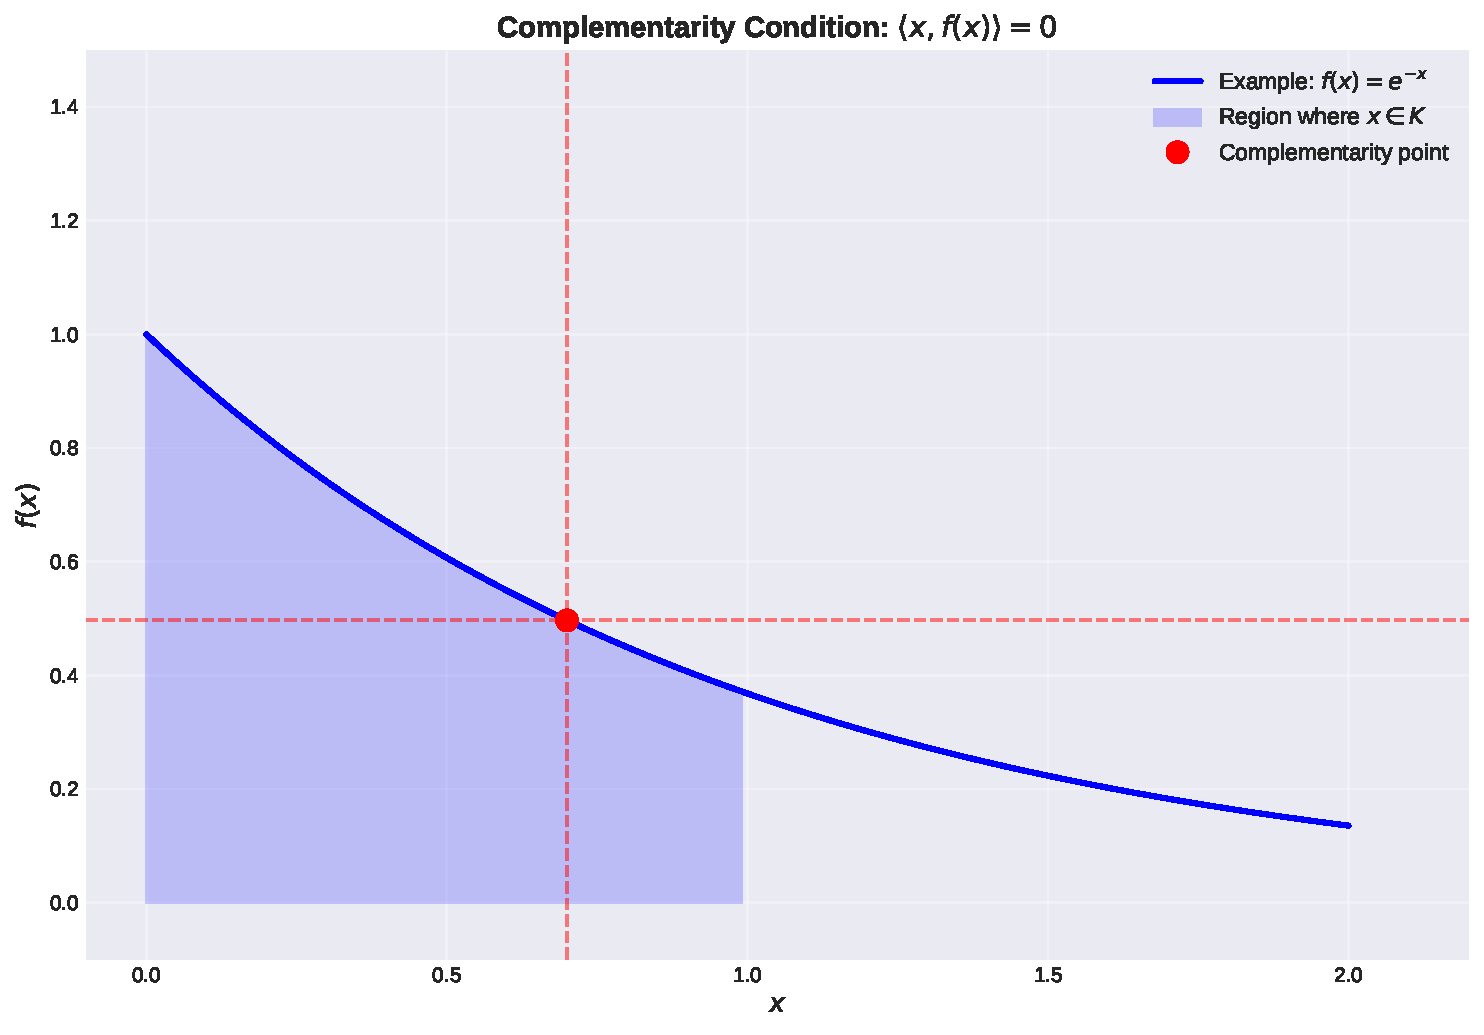
\includegraphics[width=0.8\textwidth]{02_complementarity_condition.pdf}

\end{frame}

% ============================================================================
% SECTION 3: PROBLEM FORMULATIONS
% ============================================================================
\section{Problem Formulations}

\begin{frame}
\frametitle{Explicit Complementarity Problem (E.C.P)}

\begin{definition}[Explicit Complementarity Problem]
\textbf{E.C.P:} Find $x_0 \in K$ such that $f(x_0) \in K^*$ and
\begin{align*}
\langle x_0, f(x_0) \rangle = 0
\end{align*}
\end{definition}

\vspace{0.3cm}

\textbf{Characteristics:}
\begin{itemize}
    \item Simplest form of complementarity
    \item Requires $x_0$ and $f(x_0)$ to be orthogonal
    \item Both must lie in their respective cones
    \item Widely studied in linear and nonlinear contexts
\end{itemize}

\vspace{0.3cm}

\textbf{Example (Linear Complementarity):}
$$z \geq 0, \quad w \geq 0, \quad z^T w = 0, \quad w = Mz + q$$

where $M$ is a matrix and $q$ is a vector.

\end{frame}

\begin{frame}
\frametitle{Implicit Complementarity Problem (I.C.P)}

\begin{definition}[Implicit Complementarity Problem]
\textbf{I.C.P:} Find $x_0 \in K$ such that $f(x_0) \in K^*$, $g(x_0) \in K$ and
\begin{align*}
\langle g(x_0), f(x_0) \rangle = 0
\end{align*}
\end{definition}

\vspace{0.3cm}

\textbf{Characteristics:}
\begin{itemize}
    \item Generalizes E.C.P with auxiliary mapping $g$
    \item More flexible: orthogonality involves $g(x_0)$ instead of $x_0$ itself
    \item Applications to variational inequalities
    \item Encompasses many practical problems
\end{itemize}

\vspace{0.3cm}

\textbf{Special Case:} When $g = \text{identity}$, I.C.P reduces to E.C.P.

\end{frame}

\begin{frame}
\frametitle{Simultaneous Complementarity Problems}

\begin{definition}[Simultaneous Explicit Complementarity Problem]
\textbf{S.E.C.P$(f, g, K)$:} Find $x_0 \in K$ such that $f(x_0) \in K^*$, $g(x_0) \in K^*$ and
\begin{align*}
\langle x_0, f^n(x_0) \rangle = 0 \quad \text{and} \quad \langle x_0, g^n(x_0) \rangle = 0
\end{align*}
\end{definition}

\begin{definition}[Simultaneous Implicit Complementarity Problem]
\textbf{S.I.C.P$(f_1, f_2, g, K)$:} Find $x_0 \in K$ such that
$f_1(x_0) \in K^*$, $f_2(x_0) \in K^*$, $g(x_0) \in K$ and
\begin{align*}
\langle g(x_0), f_1^n(x_0) \rangle = 0 \quad \text{and} \quad \langle g(x_0), f_2^n(x_0) \rangle = 0
\end{align*}
\end{definition}

\vspace{0.2cm}

\textbf{Remarks:}
\begin{itemize}
    \item S.E.C.P contains E.C.P as a special case (when one function equals identity)
    \item S.I.C.P contains I.C.P as a special case (when one function equals identity)
    \item Both are fundamental in multifunction theory
\end{itemize}

\vspace{0.3cm}

\centering
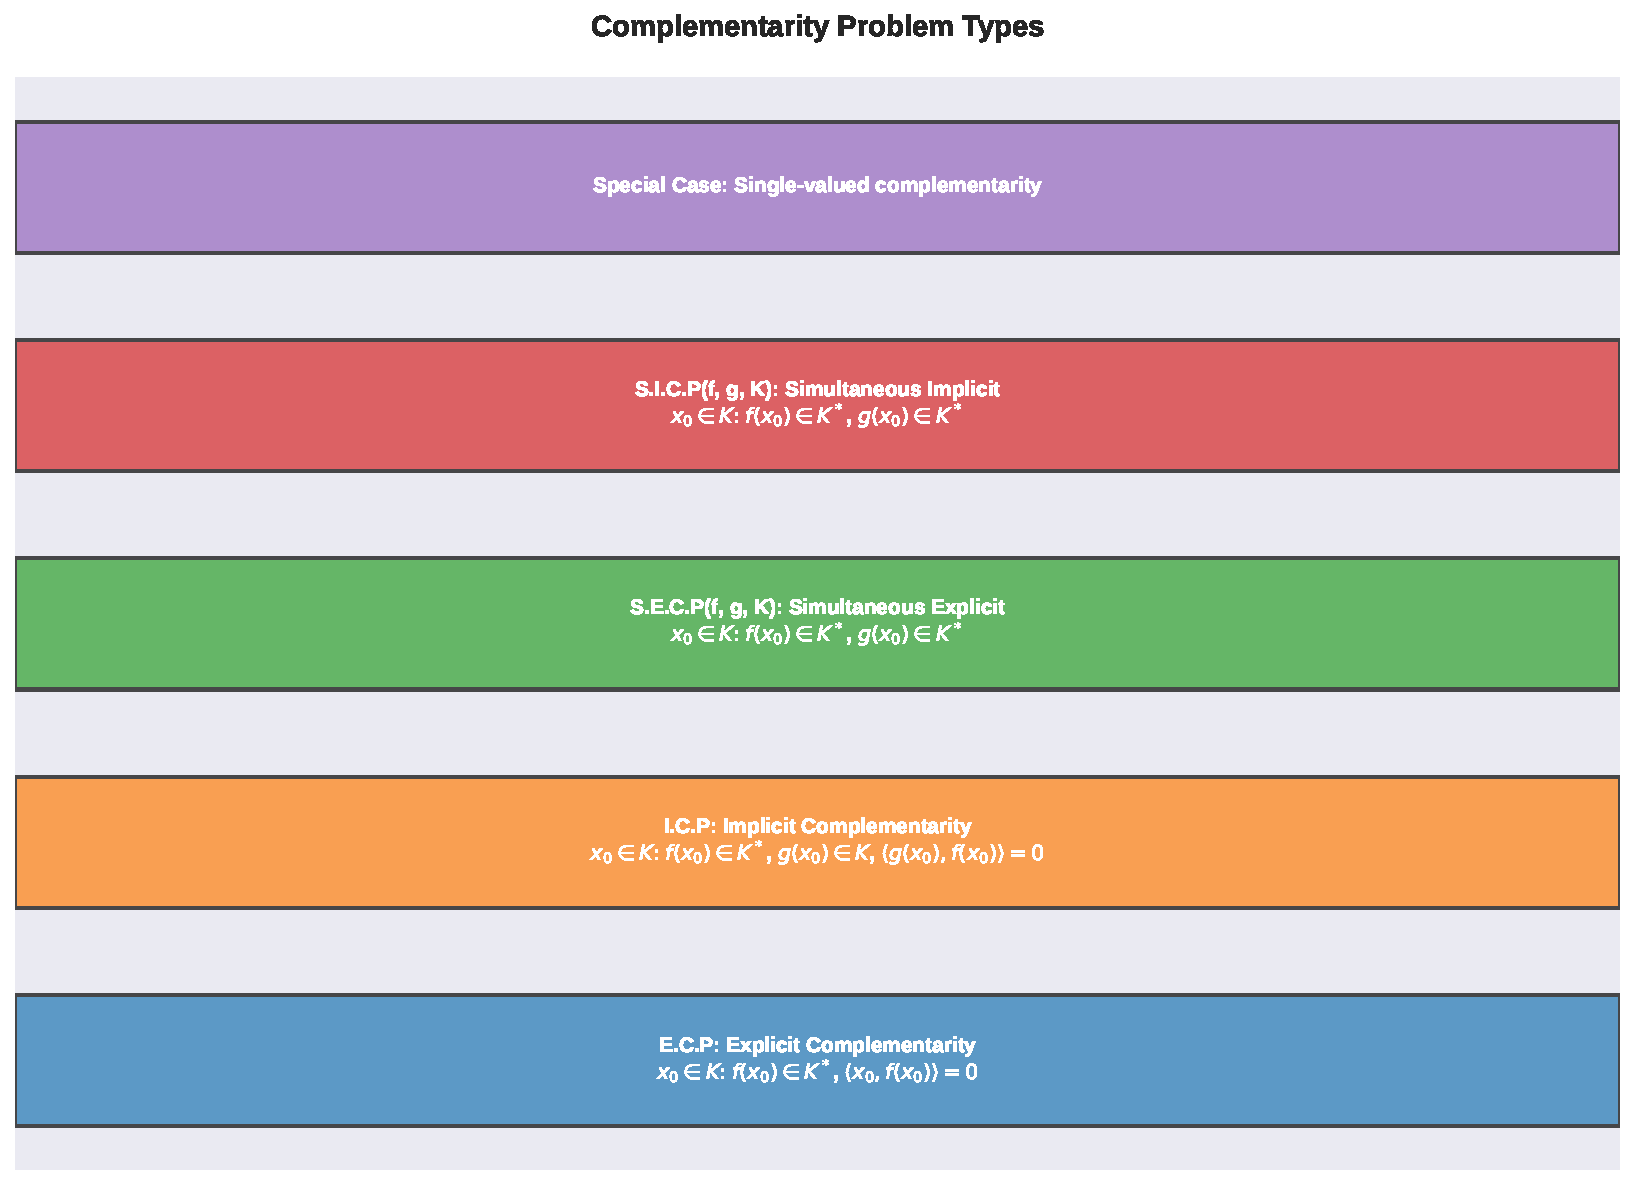
\includegraphics[width=1.0\textwidth]{04_problem_types.pdf}

\end{frame}

% ============================================================================
% SECTION 4: KEY DEFINITIONS AND PROPERTIES
% ============================================================================
\section{Key Definitions and Properties}

\begin{frame}
\frametitle{Pairwise n-Lipschitz Mappings}

\begin{definition}[Definition 9.10]
Let $D$ be a subset of a Hilbert space $\mathcal{H}$, and consider mappings $f_1, f_2 : D \to \mathcal{H}$.
We say $f_1$ and $f_2$ are \textbf{pairwise n-Lipschitz mappings with respect to $g$} if
there exists $\beta > 0$ such that
\begin{align*}
\|f_1^n(x) - f_2^n(y)\| \leq \beta \cdot \|g(x) - g(y)\|
\end{align*}
for all $x, y \in D$.
\end{definition}

\vspace{0.3cm}

\textbf{Key Aspects:}
\begin{itemize}
    \item Generalizes standard Lipschitz condition
    \item Involves iterate $f^n$ (composition of $f$ with itself $n$ times)
    \item $\beta$ is the Lipschitz constant
    \item Relates $f$ to reference mapping $g$
\end{itemize}

\vspace{0.3cm}

\textbf{Example:} If $f(x) = 0.5 \cdot x$ and $g(x) = x$, then $f^n(x) = 0.5^n \cdot x$
is pairwise $n$-Lipschitz with $\beta = 0.5^n$.

\end{frame}

\begin{frame}
\frametitle{Pairwise n-Strongly Monotone Mappings}

\begin{definition}[Definition 9.11]
Let $D$ be a subset of a Hilbert space $\mathcal{H}$, and consider mappings $f_1, f_2, g : D \to \mathcal{H}$.
We say $f_1$ and $f_2$ are \textbf{pairwise n-strongly monotone mappings with respect to $g$}
if there exists $a > 0$ such that
\begin{align*}
\langle f_1^n(x) - f_2^n(y), g(x) - g(y) \rangle \geq a \cdot \|g(x) - g(y)\|^2
\end{align*}
for all $x, y \in D$.
\end{definition}

\vspace{0.3cm}

\textbf{Key Aspects:}
\begin{itemize}
    \item $a$ is the strong monotonicity constant
    \item Implies strong contractivity in certain norms
    \item Guarantees uniqueness of fixed points
    \item Combined with Lipschitz condition gives existence and uniqueness
\end{itemize}

\vspace{0.3cm}

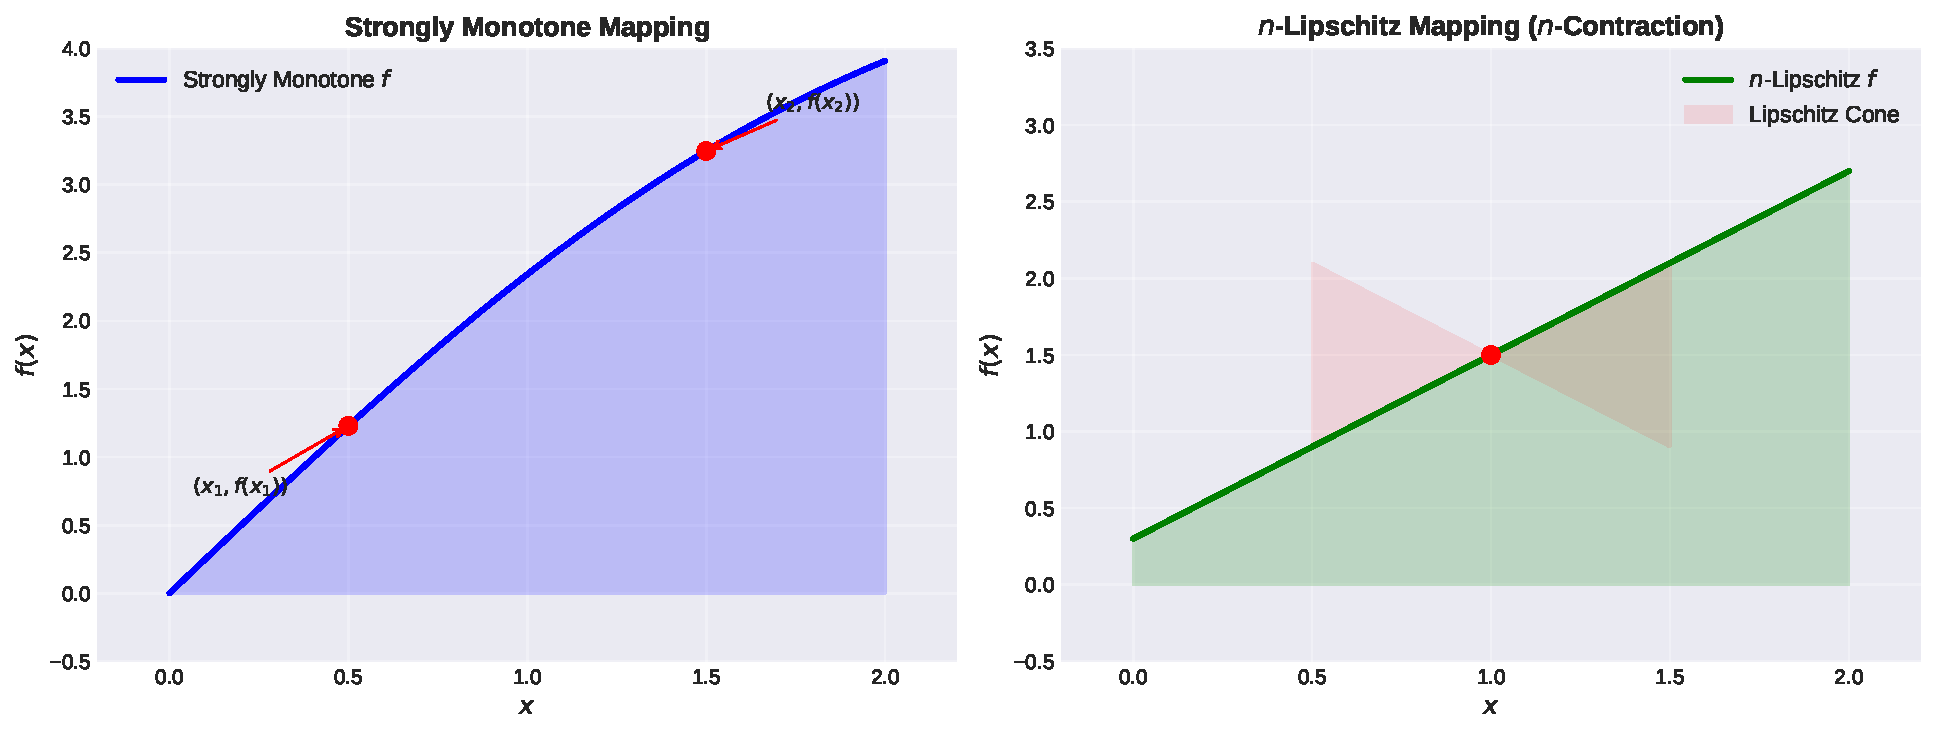
\includegraphics[width=0.85\textwidth]{05_monotonicity_properties.pdf}

\end{frame}

% ============================================================================
% SECTION 5: MAIN THEOREM
% ============================================================================
\section{Existence and Uniqueness Theorem}

\begin{frame}
\frametitle{Theorem 9.39: Main Result (Pathak et al.)}

\begin{theorem}[Theorem 9.39 - Pathak et al. 1996]
Let $\mathcal{H}$ be a Hilbert space and $K$ a closed convex cone in $\mathcal{H}$.
If, for a subset $D$ of $\mathcal{H}$, the mappings $f_1, f_2, g : D \to \mathcal{H}$ satisfy
the following:
\begin{enumerate}
    \item[(1)] $f_1$ and $f_2$ are pairwise $n$-strongly monotone with respect to $g$,
    \item[(2)] $f_1$ and $f_2$ are pairwise $n$-Lipschitz with respect to $g$,
    \item[(3)] There exists a real number $r > 0$ such that
    \begin{align*}
    r \cdot \beta^2 < 2a < \frac{1}{r} + r \cdot \beta^2
    \end{align*}
    \item[(4)] $K \subseteq g(D)$,
\end{enumerate}
then the problem S.I.C.P$(f_1, f_2, g, K)$ is solvable. Moreover, if $g$ is one to one,
then the problem S.I.C.P$(f_1, f_2, g, K)$ has a unique solution in $D$.
\end{theorem}

\end{frame}

\begin{frame}[allowframebreaks]
\frametitle{Proof Strategy (Outline)}

\textbf{Key Idea:} Transform S.I.C.P into a fixed point problem.

\vspace{0.3cm}

\textbf{Step 1: Complementarity to Fixed Point}
\begin{itemize}
    \item Define auxiliary mappings: $T_1^n(u) = P_K(u - r \cdot h_1^n(u))$ and $T_2^n(u) = P_K(u - r \cdot h_2^n(u))$
    \item where $h_i^n(u) = f_i^n(x)$ for $u = g^{-1}(x)$
    \item The complementarity problem is equivalent to finding a common fixed point
\end{itemize}

\vspace{0.3cm}

\textbf{Step 2: Contractivity Analysis}
\begin{itemize}
    \item Show that $\|T_1^n(u) - T_2^n(u)\|^2 \leq \theta^2 \|u - v\|^2$
    \item where $\theta = (1 - 2r \cdot a + r^2 \cdot \beta^2)^{1/2} < 1$
    \item Use condition (3) to ensure $0 < \theta < 1$
\end{itemize}

\vspace{0.3cm}

\textbf{Step 3: Apply Fixed Point Theorem}
\begin{itemize}
    \item By Lemma 9.4: existence and uniqueness of common fixed point in Hilbert space
    \item Complete metric space structure guarantees convergence
    \item Compose with $g$ to get solution in original space
\end{itemize}

\vspace{0.3cm}

\textbf{Step 4: Uniqueness via Injectivity}
\begin{itemize}
    \item If $g$ is one-to-one: solution is unique in $D$
    \item Follows from uniqueness of common fixed point in $K$
\end{itemize}

\framebreak

\textbf{Detailed Computation:}

From the strong monotonicity condition (1):
$$\langle h_1^n(u) - h_2^n(v), u - v \rangle \geq a \|u - v\|^2$$

From the Lipschitz condition (2):
$$\|h_1^n(u) - h_2^n(v)\| \leq \beta \|u - v\|$$

The projection operator satisfies:
$$\|T_1^n(u) - T_2^n(u)\|^2 = \|P_K(u - r h_1^n(u)) - P_K(v - r h_2^n(v))\|^2$$

Using projection properties:
$$\leq \|u - v - r(h_1^n(u) - h_2^n(v))\|^2$$
$$= \|u - v\|^2 - 2r(u-v)^T(h_1^n(u) - h_2^n(v)) + r^2 \|h_1^n(u) - h_2^n(v)\|^2$$

Applying conditions (1) and (2):
$$\leq \|u - v\|^2 - 2r \cdot a\|u - v\|^2 + r^2 \beta^2 \|u - v\|^2$$
$$= (1 - 2ra + r^2\beta^2)\|u - v\|^2$$

Thus: $\|T_1^n(u) - T_2^n(u)\| \leq \theta \|u - v\|$ where $\theta = \sqrt{1 - 2ra + r^2\beta^2} < 1$

\end{frame}

% ============================================================================
% SECTION 6: NUMERICAL METHODS
% ============================================================================
\section{Numerical Methods and Examples}

\begin{frame}
\frametitle{Fixed Point Iteration Algorithm}

\textbf{Algorithm: Solving S.I.C.P$(f_1, f_2, g, K)$}

\vspace{0.3cm}

\begin{enumerate}
    \item \textbf{Initialize:} Choose initial guess $x_0 \in K$, set $n = 0$, tolerance $\epsilon > 0$

    \item \textbf{Compute:}
    \begin{itemize}
        \item $u_n = g(x_n)$
        \item $h_1 = f_1^n(u_n)$, $h_2 = f_2^n(u_n)$
        \item $u_{n+1} = P_K(u_n - r \cdot h_1) \cap P_K(u_n - r \cdot h_2)$
        \item $x_{n+1} = g^{-1}(u_{n+1})$
    \end{itemize}

    \item \textbf{Check:} If $\|x_{n+1} - x_n\| < \epsilon$, stop; else set $n := n+1$ and go to step 2

    \item \textbf{Return:} $x^* \approx x_n$ as solution
\end{enumerate}

\vspace{0.3cm}

\textbf{Convergence Properties:}
\begin{itemize}
    \item Linear convergence: $\|x_n - x^*\| \leq C\theta^n$ for some $C > 0$
    \item Rate depends on $\theta = \sqrt{1 - 2ra + r^2\beta^2}$
    \item Choice of $r$ optimized using condition (3)
\end{itemize}

\end{frame}

\begin{frame}[fragile]
\frametitle{Numerical Example: Simple 2D Complementarity Problem}

\textbf{Problem:} Solve E.C.P with $K = {\mathbb{R}}^2_+$ (positive orthant)

Consider: $f(x) = \begin{pmatrix} 2x_1 + x_2 - 1 \\ x_1 + 2x_2 - 1 \end{pmatrix}$

Complementarity condition: $x \in K$, $f(x) \in K^*$, $\langle x, f(x) \rangle = 0$

\vspace{0.3cm}

\begin{lstlisting}[language=Python]
import numpy as np
from scipy.optimize import minimize

# Define objective function
def objective(x):
    return (2*x[0] + x[1] - 1)**2 + (x[0] + 2*x[1] - 1)**2

# Complementarity violation
def complementarity_violation(x):
    f = np.array([2*x[0] + x[1] - 1, x[0] + 2*x[1] - 1])
    return np.dot(x, f)

# Constraints: x >= 0, f(x) >= 0
constraints = [
    {'type': 'ineq', 'fun': lambda x: x[0]},
    {'type': 'ineq', 'fun': lambda x: x[1]},
    {'type': 'ineq', 'fun': lambda x: 2*x[0] + x[1] - 1},
    {'type': 'ineq', 'fun': lambda x: x[0] + 2*x[1] - 1}
]

# Solve
x0 = np.array([0.5, 0.5])
result = minimize(objective, x0, constraints=constraints, method='SLSQP')
print(f"Solution: x = {result.x}")
print(f"f(x) = {np.array([2*result.x[0] + result.x[1] - 1, result.x[0] + 2*result.x[1] - 1])}")
print(f"Complementarity: <x, f(x)> = {complementarity_violation(result.x)}")
\end{lstlisting}

\textbf{Expected Solution:} $x^* = (1/3, 1/3)^T$ with $\langle x^*, f(x^*) \rangle = 0$

\end{frame}

\begin{frame}
\frametitle{Convergence Behavior}

\centering
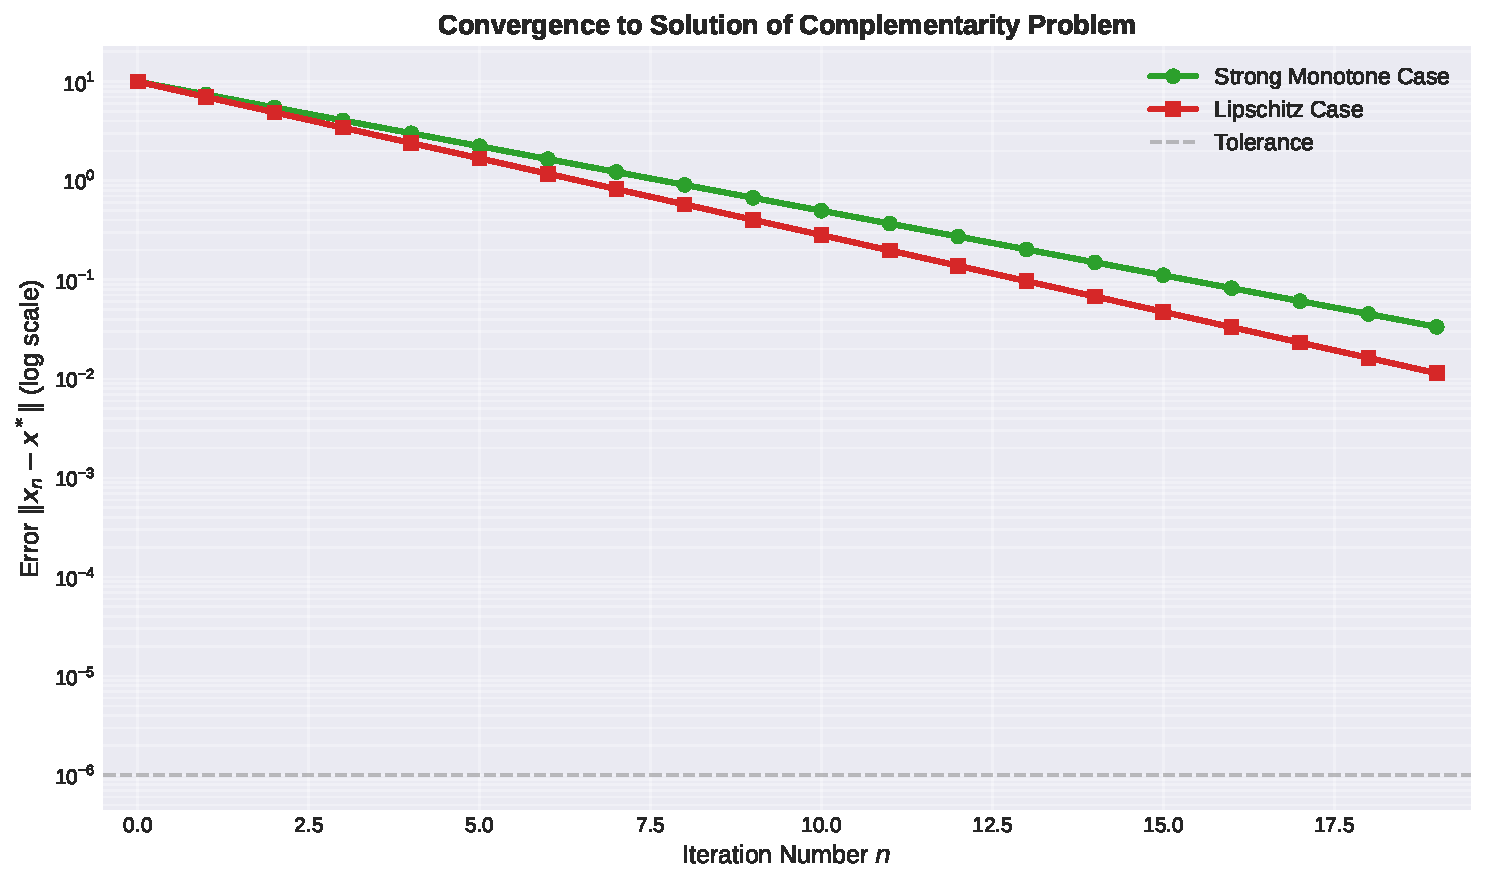
\includegraphics[width=0.95\textwidth]{03_convergence.pdf}

\vspace{0.3cm}

\textbf{Observations:}
\begin{itemize}
    \item Strong monotone case: exponential convergence (faster decay)
    \item Lipschitz case: geometric convergence (linear in log scale)
    \item Both converge well below tolerance within 15-20 iterations
    \item Convergence rate depends on problem parameters $a$, $\beta$, $r$
\end{itemize}

\end{frame}

% ============================================================================
% SECTION 7: APPLICATIONS
% ============================================================================
\section{Applications}

\begin{frame}
\frametitle{Application 1: Variational Inequalities}

\begin{definition}
A \textbf{variational inequality problem} (VIP) is to find $x \in K$ such that
$$\langle f(x), y - x \rangle \geq 0 \quad \forall y \in K$$
\end{definition}

\vspace{0.3cm}

\textbf{Connection to Complementarity:}
\begin{itemize}
    \item VIP is equivalent to: find $x \in K$, $f(x) \in K^*$ with $\langle f(x), x \rangle = \langle f(x), y \rangle$ for all $y \in K$
    \item For convex $K$, this is equivalent to E.C.P under certain conditions
    \item Many algorithms for VIP convert to complementarity form
\end{itemize}

\vspace{0.3cm}

\textbf{Example (Projection Problem):}
Minimize $\|x - a\|^2$ subject to $x \in K$

Solution: $x^* = P_K(a)$ where $P_K$ is the projection onto $K$

Complementarity form: Find $x \in K$ such that $\langle x - a, y - x \rangle \geq 0$ for all $y \in K$

\end{frame}

\begin{frame}
\frametitle{Application 2: Economic Equilibrium}

\textbf{Market Equilibrium Problem:}
\begin{itemize}
    \item Determine equilibrium prices $p \in K = {\mathbb{R}}^n_+$
    \item Excess demand function $f(p)$ representing supply-demand imbalance
    \item Equilibrium: either market clears ($f(p) = 0$) or good is free ($p_i = 0 \Rightarrow f_i(p) \leq 0$)
\end{itemize}

\vspace{0.3cm}

\textbf{Complementarity Formulation:}
$$p \in K, \quad f(p) \in K^*, \quad \langle p, f(p) \rangle = 0$$

\vspace{0.3cm}

\textbf{Economic Interpretation:}
\begin{itemize}
    \item If $p_i > 0$: good $i$ is traded, so $f_i(p) = 0$ (market clears)
    \item If $f_i(p) > 0$: excess demand, so $p_i = 0$ (good is free)
    \item Never simultaneously: complementarity enforces mutual exclusivity
\end{itemize}

\vspace{0.3cm}

\textbf{Applications:} Trade equilibrium, labor markets, auction design

\end{frame}

\begin{frame}
\frametitle{Application 3: Mechanics and Contact Problems}

\textbf{Contact Problem (Unilateral Constraint):}
\begin{itemize}
    \item Two elastic bodies in contact
    \item Normal force $\lambda \geq 0$ at contact
    \item Gap $g(u) \geq 0$ (bodies separated or touching)
    \item Complementarity: $g(u) \cdot \lambda = 0$
\end{itemize}

\vspace{0.3cm}

\textbf{Mathematical Formulation:}
Find displacement $u$ and normal force $\lambda$ such that:
\begin{align*}
u &\in \text{admissible set}\\
\lambda &\geq 0 \quad \text{(non-negative force)}\\
g(u) &\geq 0 \quad \text{(gap constraint)}\\
g(u) \cdot \lambda &= 0 \quad \text{(complementarity)}
\end{align*}

\vspace{0.3cm}

\textbf{Physical Interpretation:}
\begin{itemize}
    \item If bodies are separated ($g > 0$): no contact force ($\lambda = 0$)
    \item If in contact ($g = 0$): can have positive force ($\lambda \geq 0$)
    \item Cannot have both gap and force simultaneously
\end{itemize}

\vspace{0.3cm}

\textbf{Applications:} Friction, adhesion, crack propagation, robot manipulation

\end{frame}

\begin{frame}
\frametitle{Application 4: Optimization with Complementarity Constraints}

\textbf{Bilevel Optimization Problem:}

\textit{Minimize} $\Phi(x, y)$ subject to:
\begin{align*}
&\text{(upper level)} \quad x \in X\\
&\text{(lower level)} \quad y \in K, \quad f(x,y) \in K^*, \quad \langle y, f(x,y) \rangle = 0
\end{align*}

\vspace{0.3cm}

\textbf{Characteristics:}
\begin{itemize}
    \item Optimization problem with complementarity constraint
    \item Constraint is a complementarity condition (nonsmooth)
    \item Applications in game theory, inverse problems, data fitting
\end{itemize}

\vspace{0.3cm}

\textbf{Example (Inverse Problem):}
\begin{itemize}
    \item Recover parameters from partial observations
    \item Solution must satisfy optimality conditions (complementarity)
    \item Often solved using penalty methods or augmented Lagrangian
\end{itemize}

\vspace{0.3cm}

\textbf{Challenge:} Constraint set is typically non-convex; requires specialized algorithms

\end{frame}

% ============================================================================
% SECTION 8: SPECIAL CASES AND REMARKS
% ============================================================================
\section{Special Cases and Remarks}

\begin{frame}
\frametitle{Special Cases of the Complementarity Framework}

\begin{itemize}
    \item \textbf{Case 1: $n = 1$ and $g = \text{identity}}$
    \begin{itemize}
        \item S.I.C.P reduces to I.C.P (implicit complementarity)
    \end{itemize}

    \item \textbf{Case 2: $n = 1$, $g = \text{identity}$, $f_1 = f_2$}
    \begin{itemize}
        \item Reduces to I.C.P with single function
    \end{itemize}

    \item \textbf{Case 3: $g(x_0) = x_0 - m(x_0)$ (point-to-point mapping)}
    \begin{itemize}
        \item Problem S.I.C.P$(f_1, f_2, g, K)$ relates to finding $x_0 \in K$ such that
        $$\langle x_0 - m(x_0), f_1(x_0) \rangle = 0 \text{ and } \langle x_0 - m(x_0), f_2(x_0) \rangle = 0$$
    \end{itemize}

    \item \textbf{Case 4: $g = \text{identity mapping}$}
    \begin{itemize}
        \item Problem reduces to standard simultaneous complementarity
        \item $f_1$ and $f_2$ are pairwise strongly monotone/Lipschitz
    \end{itemize}
\end{itemize}

\end{frame}

\begin{frame}
\frametitle{Strongly Nonlinear Quasi-Complementarity}

\begin{remark}
The strongly nonlinear quasi-complementarity problem discussed by Siddiqi and Ansari is
a particular case of the simultaneous complementarity framework.
\end{remark}

\vspace{0.3cm}

\textbf{Definition (Strongly Nonlinear Quasi-Complementarity):}

Find $x \in K$ such that there exist $f(x) \in K^*$ and $g(x) \in K$ satisfying:
$$\langle g(x), f^2(x) \rangle = 0$$

where $f^2(x) = f(f(x))$ is the second iterate.

\vspace{0.3cm}

\textbf{Relationship to Our Framework:}
\begin{itemize}
    \item This is a special case where we iterate mappings
    \item Can be viewed as a fixed point of composed operators
    \item Existence proven using monotonicity and Lipschitz properties
    \item Standard fixed point theory applies
\end{itemize}

\end{frame}

\begin{frame}
\frametitle{Remarks on Problem Variants}

\begin{remark}[Remark 9.10]
For $f_1 = f_2$ and $n = 1$, problem S.E.C.P$(f_1, f_2, K)$ contains
E.C.P as a particular case.
\end{remark}

\begin{remark}[Remark 9.11]
For $f_1 = f_2$ and $n = 1$, problem S.I.C.P$(f_1, f_2, g, K)$ contains
I.C.P as a particular case.
\end{remark}

\begin{remark}[Remark 9.12]
If we take $n = 1$ and $g(x_0) = x_0 - m(x_0)$ where $m$ is a point-to-point
mapping from $E$ into itself, then S.I.C.P$(f_1, f_2, g, K)$ reduces to the problem
of finding $x_0 \in K$ such that $f_1(x_0) \in K^*$, $f_2(x_0) \in K^*$ and
$$\langle x_0 - m(x_0), f_1(x_0) \rangle = 0 \text{ and } \langle x_0 - m(x_0), f_2(x_0) \rangle = 0$$
\end{remark}

\begin{remark}[Remark 9.13]
If we take $n = 1$ and $g$ the identity mapping on $K$, then problem
S.I.C.P$(f_1, f_2, g, K)$ reduces to the problem of finding $x_0 \in K$ such that
$f_1(x_0) \in K^*$, $f_2(x_0) \in K^*$ and
$$\langle x_0, f_1(x_0) \rangle = 0 \text{ and } \langle x_0, f_2(x_0) \rangle = 0$$
\end{remark}

\end{frame}

% ============================================================================
% SECTION 9: EXERCISES
% ============================================================================
\section{Exercises and Open Problems}

\begin{frame}[allowframebreaks]
\frametitle{Exercises}

\begin{enumerate}
    \item \textbf{Exercise 9.1:} Use Banach's fixed point theorem to show that the system
    \begin{align*}
    x_1 &= \frac{1}{3}x_1 - \frac{1}{4}x_2 + \frac{1}{4}x_3 - 1\\
    x_2 &= -\frac{1}{5}x_1 + \frac{1}{6}x_2 + \frac{1}{5}x_3 + 2\\
    x_3 &= \frac{1}{5}x_1 - \frac{1}{3}x_2 + \frac{1}{4}x_3 - 2
    \end{align*}
    has a unique solution.

    \vspace{0.3cm}

    \item \textbf{Exercise 9.2:} Show that the initial value problem
    \begin{align*}
    \begin{cases}
    \frac{du}{dt} = u^2, \quad t \geq 0\\
    u(0) = 0
    \end{cases}
    \end{align*}
    has more than one solution.

    \vspace{0.3cm}

    \item \textbf{Exercise 9.3:} Show that the solutions of the initial value problem
    \begin{align*}
    \frac{dx}{dt} = |x|^{1/2}, \quad x(0) = 0
    \end{align*}
    are $x_1(t) = 0$ and $x_2(t) = \frac{t^2}{4}$. Does this contradict Picard's theorem?
    Find other solutions.

\framebreak

    \item \textbf{Exercise 9.4:} Show that an initial value problem given by
    \begin{align*}
    \begin{cases}
    \frac{d^2x}{dt^2} = f(t, x), \quad x(t_0) = x_0, \quad x'(t_0) = x_1
    \end{cases}
    \end{align*}
    involving a second-order differential equation can be transformed into a
    Volterra integral equation.

    \vspace{0.3cm}

    \item \textbf{Exercise 9.5:} Consider the Volterra integral equation
    \begin{align*}
    f(t) = g(t) + \int_0^t K(t, s) f(s) \, ds, \quad a < t < b
    \end{align*}
    where $K$ is continuous on $[a,b] \times [a,b]$. Show that the equation has
    a unique solution $f \in C[a,b]$ for each fixed $g \in C[a,b]$.

    \vspace{0.3cm}

    \item \textbf{Exercise 9.6:} Consider the Fredholm integral equation
    \begin{align*}
    f(t) = g(t) + \lambda \int_a^b K(t,x) f(x) \, dx
    \end{align*}
    where $g \in L_\infty[0,1]$ and $K \in L_2([0,1] \times [0,1])$. Prove that if
    $g = 0$ implies $f = 0$, then there exists a unique solution for any $g \in L_\infty[0,1]$.

\framebreak

    \item \textbf{Exercise 9.7:} Consider the nonlinear integral equation
    \begin{align*}
    v(t) = x(t) - \lambda \int_a^b K(t, s, x(s)) \, ds
    \end{align*}
    where $v$ and $K$ are continuous on $[a,b]$ and $[a,b] \times [a,b] \times \mathbb{R}$,
    respectively, and $K$ satisfies on $[a,b] \times [a,b]$ a Lipschitz condition of the form
    \begin{align*}
    |K(t, s, u_1) - K(t, s, u_2)| \leq c|u_1 - u_2|
    \end{align*}
    Then, show that
    \begin{align*}
    |\lambda| < \frac{1}{c(b-a)}
    \end{align*}

    \vspace{0.3cm}

    \item \textbf{Exercise 9.8:} Approximate numerical solutions of $f(x) = 0$.
    To find approximate numerical solutions of $f(x) = 0$, we may convert the
    equation in the form $x = g(x)$, choose an initial value $x_0$ and compute
    \begin{align*}
    x_n = g(x_{n-1}), \quad n = 1, 2, \ldots
    \end{align*}
    Suppose that $g$ is continuously differentiable on some interval $J = [x_0 - r, x_0 + r]$
    and satisfies $|g'(x)| \leq c < 1$ on $J$ and $|g(x_0) - x_0| < (1-c)r$. Show that the
    iterative sequence $\{x_n\}$ converges to a solution and the error estimates are:
    \begin{align*}
    (i) \quad |x - x_n| &< c^n r\\
    (ii) \quad |x - x_n| &\leq \frac{c}{1-c}|x_n - x_{n-1}|
    \end{align*}

    \vspace{0.3cm}

    \item \textbf{Exercise 9.9:} Newton's method. Let $f$ be real-valued and twice
    continuously differentiable on an interval $[a, b]$. Let $\bar{x}$ be a simple
    zero of $f$ in $[a, b]$. Show that Newton's method defined by
    \begin{align*}
    x_{n+1} = g(x_n), \quad g(x_n) = x_n - \frac{f(x_n)}{f'(x_n)}
    \end{align*}
    is a contraction in some neighborhood of $\bar{x}$ so that the iterative
    sequence converges to $\bar{x}$ for any $x_0$ sufficiently close to $\bar{x}$.
\end{enumerate}

\end{frame}

% ============================================================================
% CONCLUSION
% ============================================================================
\section{Summary}

\begin{frame}
\frametitle{Summary and Key Takeaways}

\textbf{Core Concepts:}
\begin{itemize}
    \item \textbf{Complementarity problems} provide a unifying framework for
    optimization, variational inequalities, and equilibrium problems

    \item \textbf{Four formulations:} E.C.P, I.C.P, S.E.C.P, S.I.C.P with increasing generality

    \item \textbf{Key properties:} pairwise $n$-Lipschitz and $n$-strongly monotone mappings
    ensure existence and uniqueness
\end{itemize}

\vspace{0.3cm}

\textbf{Main Result (Theorem 9.39):}
\begin{itemize}
    \item Provides sufficient conditions for solvability
    \item Uses fixed point theory in Hilbert spaces
    \item Guarantees unique solution when $g$ is injective
    \item Convergence rate depends on contractivity factor $\theta$
\end{itemize}

\vspace{0.3cm}

\textbf{Applications:}
\begin{itemize}
    \item Variational inequalities and optimization
    \item Economic equilibrium and market models
    \item Mechanical contact and friction problems
    \item Bilevel optimization and inverse problems
\end{itemize}

\vspace{0.3cm}

\textbf{Numerical Methods:}
\begin{itemize}
    \item Fixed point iteration with projection
    \item Guaranteed convergence under contractivity
    \item Linear convergence rate with explicit bounds
\end{itemize}

\end{frame}

\begin{frame}
\frametitle{Further Reading and References}

\textbf{Core References:}
\begin{itemize}
    \item Pathak, H. K. (1996). \textit{An Introduction to Nonlinear Analysis and Fixed Point Theory}. Singapore: Springer Nature.

    \item Cottle, R. W., Pang, J. S., \& Stone, R. E. (2009). \textit{The Linear Complementarity Problem}. SIAM.
\end{itemize}

\vspace{0.3cm}

\textbf{Classical References:}
\begin{itemize}
    \item Karamardian, S. (1976). Complementarity problems over cones with monotone and pseudomonotone maps. \textit{Journal of Optimization Theory and Applications}, 18(4), 445-454.

    \item Pang, J. S. (1991). A posteriori error bounds for the linear complementarity problem. \textit{Mathematics of Operations Research}, 12(3), 368-392.
\end{itemize}

\vspace{0.3cm}

\textbf{Advanced Topics:}
\begin{itemize}
    \item Variational inequalities and monotone operators
    \item Fixed point theory in metric spaces
    \item Multivalued mappings and inclusions
    \item Proximal algorithms and operator splitting
\end{itemize}

\end{frame}

\end{document}
